
\documentclass[12pt,journal]{IEEEtran}
\usepackage{graphicx}
\usepackage{placeins}
\usepackage{listings}
\usepackage{color}
\usepackage{multicol}
\usepackage{array}
\usepackage{setspace}
\usepackage{lipsum}
\usepackage{makecell,interfaces-makecell}
\usepackage{caption}
\usepackage{biblatex}
\usepackage{fancyhdr}


\graphicspath{ {./Images/} }


\ifCLASSINFOpdf
  % \usepackage[pdftex]{graphicx}
  % declare the path(s) where your graphic files are
  % \graphicspath{{../pdf/}{../jpeg/}}
  % and their extensions so you won't have to specify these with
  % every instance of \includegraphics
  % \DeclareGraphicsExtensions{.pdf,.jpeg,.png}
\else
  % or other class option (dvipsone, dvipdf, if not using dvips). graphicx
  % will default to the driver specified in the system graphics.cfg if no
  % driver is specified.
  % \usepackage[dvips]{graphicx}
  % declare the path(s) where your graphic files are
  % \graphicspath{{../eps/}}
  % and their extensions so you won't have to specify these with
  % every instance of \includegraphics
  % \DeclareGraphicsExtensions{.eps}
\fi

% correct bad hyphenation here
\hyphenation{op-tical net-works semi-conduc-tor}



\begin{document}
\begin{titlepage}
    \begin{center}
        \vspace*{1cm}
 
        \Huge
        \textbf{Arduino Based Computer Controlling Using HandGestures}
 
        \vspace{0.1cm}
        \LARGE
        Final Project Documentation\\
        Done By\\
        \vspace{1.5cm}
 
        \textbf{ Teegapuram Deepika Reddy}
         \LARGE
         \\ 
         Graduate Student\\
         Student ID: 200415938
        \vspace{1.5cm}
 
        \includegraphics[width=0.4\textwidth]{Images/logo.PNG}
 
        \Large
        Supervised By \\
        \textbf{Tomesh Trevor }\\
        Sessional Lecturer \\
        CS-807, Interactive Hardware\\
        University of Regina \\
        April 17, 2019
 
    \end{center}
\end{titlepage}

\tableofcontents


% paper title
% can use linebreaks \\ within to get better formatting as desired
% Do not put math or special symbols in the title.

\title{Arduino Based Computer Controlling Using Hand Gestures}


\author{Deepika Teegapuram, Student ID: 200415938,~\IEEEmembership{Graduate Student,~University~of~Regina}
        %other authors go below
        %Bob~Builder,~\IEEEmembership{Student,~University~of~Regina,}
        %and~Noob~McScrubb,~\IEEEmembership{Student,~University~of~Regina}
        }
\onecolumn



% The paper headers
% This should either be the name of the journal or the 
% first four(ish) words of the paper
\markboth{Arduino Based Gesture Controlling,project report, Apr~07~2019}%
{Shell \MakeLowercase{\textit{et al.}}: Design, Template, Computer Science }
% The only time the second header will appear is for the odd numbered pages
% after the title page when using the twoside option.


% make the title area
\maketitle

% As a general rule, do not put math, special symbols or citations
% in the abstract or keywords.

% Note that keywords are not normally used for peerreview papers.


% For peer review papers, you can put extra information on the cover
% page as needed:
% \ifCLASSOPTIONpeerreview
% \begin{center} \bfseries EDICS Category: 3-BBND \end{center}
% \fi
%
% For peerreview papers, this IEEEtran command inserts a page break and
% creates the second title. It will be ignored for other modes.
\onehalfspacing
\section{Overview}
The purpose of this paper is to make a modification to the existing project to support additional features. The source project inspired for building this project is published by Smart Technology in www.hackster.io in 2017. As a part of modifications, advanced features and flexibility are added to this project.

\section{Introduction}

% Some journals put the first two words in caps:
% \IEEEPARstart{T}{his demo} file is ....
% 
% Here we have the typical use of a "T" for an initial drop letter
% and "HIS" in caps to complete the first word.
\IEEEPARstart{T}{he} evolution of technologies over time has led to the introduction of open source platforms which provide various opportunities to approach a solution. The transformation from a room size computer to wearable compatible computers has motivated towards making of touch sensor systems which have been enhanced with absolutely no-touch required systems. This remarkable transformation to no-touch based systems i.e. sensor operating system has inspired to build this project. In this project, the effective translation between gestures and the type of operation to be performed in the computer is purely decided on the distance between the hand and the sensor.
\par Instead of using human touch required devices like Keyboard, Mouse or Joystick, the new approach of sensor-based systems will open wide opportunities to operate the computers. Nowadays, we see most of the LCD Screens are supporting Finger-Touch Technology. The idea behind this project is to build a Human Machine Interface (HMI) by reducing the Touch-Based Systems and replacing them with Sensor- Based Systems. The idea of integrating this project with Python has unveiled a new dimension to the Arduino Programming. With the support of sensors, more features can be added to improve human interaction with the computer.
\par This project is an amalgamation of Arduino and Python platforms. Arduino is considered as one of the most powerful and compatible electronics prototyping platforms. On the other hand, Python is the most advanced and widely used open source platform for high-end programming. The interaction bridge built between Arduino and Python gives the privilege to understand the distance of the hand from the sensor to reflect the respective operation in the computer.

\par This project incorporates twelve different operations in the computer on different applications which are pre-installed. To perform these operations, we require 2 Ultrasonic sensors, each sensor has its own set of distance ranges and operations to perform. The moment any object or hand interferes the waves of the sensor, the Arduino program calculates the distance at which the interference has been encountered and hands over to Python for finding out which operation to perform in the computer based on the value of the distance. 
\newpage
\par Out of the twelve operations, seven operations are being performed on the VLC Media Player, 3 operations on the Chrome Web Browser, one operation for recording a live video from the webcam installed in the laptop and finally to shut down the laptop.

% You must have at least 2 lines in the paragraph with the drop letter
% (should never be an issue)

%%%%%%%%%%%%%%%%%%%%%%%%%%%%%%%%%%%%%%%%%%%%%%%%%%%%%%%%%%%%%%%%%%%%%%%%%%%%%%%%%%%%%%%%%%%%%%%%%%%%%%%%%%%

\section{Background}

To put pen to paper, to list down the ideas to integrate Arduino and Python which opens wide doors for supporting new functionalities, we browsed for the project which supports these two platforms. One of the best results found was to control the computer using gestures. The publisher of this project has made a video which acts as a manual to trigger a sequence of the events using gestures.
\par The idea of this existing project is to implement five features on VLC Media Player. These features are unique and demonstrate their own importance and purpose. The following is the description of each feature.
\begin{enumerate}
  \item Play/Pause: By placing both the hands as near as possible to the Ultrasonic sensor will cause either Pause or play action.
  \bigskip
  \item Rewind the video: Place the hand slightly far from the leftmost Ultrasonic sensor caused the ‘Rewind’ action.
  \bigskip
  \item Forward the video: Place the hand in front of the right sensor at a specific distance.
  \bigskip
  \item Increase volume: Position the hand far from the left sensor and pull it away from the sensor.
  \bigskip
  \item Decrease volume: Position the hand at a distance far from the right sensor and push the hand toward the sensor.
\end{enumerate}
\par We must appreciate the design for minimal use of the sensors to manage to bring out these impeccable features.  The author of the existing project has given an in-detail list of the libraries which are required to start the development process. 
\par There is a specialty of each library in supporting these features. They provide user-level access to the program to access and interact with the applications on the computer. The following are the pre-requisite libraries in Python that are suggested by the author to make the existing project to work.
\begin{enumerate}
  \item The version of python should be 2.7.14 - 2.3.x.
  \item Installation of pySerial, which enabled the python to read the Serial Monitor of Arduino.
\end{enumerate}

\par The idea is to capture the distance between the hand and the sensor. The author of the existing project has come up with the thought process of capturing the distance, when the distance meets the required distance which is set up in the Arduino program, print the necessary action to be performed on the Serial Monitor.
\par The library pySerial in Python will be listening to the Serial Monitor, as soon as ¬¬the action name is printed on the Serial Monitor matches with one of the actions in the Python program, that corresponding code will be executed to perform the action.
\newpage
\par To perform the above 5 operations, the hand must interfere with the Ultrasonic sensor waves at a distance which is registered in the program. Each feature has a distance value in unique. Using the same technique, I have included the eight additional operations as an extension to this project.
\section{Materials Required}
The following are the materials required for developing this project:
\begin{itemize}
  \item Arduino UNO
  \item Ultrasonic sensors(HC-SR04)-2
  \item Connecting Wires
  \item The USB cable for connecting Arduino
  \item A Laptop
\end{itemize}

\section{Design Process}
The design process has started by keeping in mind about the number of features that are going to take place in the project. Initially, there were twenty features listed by holding on to three Ultrasonic sensors. Unfortunately, due to the scarcity of the availability of these sensors, I had to stick with two Ultrasonic sensors with the supporting features of twelve.
\par Since, the sensors are overloaded with an equal number of responsibilities to do, a detailed classification of which operation must be done at what distance of the hand from the sensor to trigger the functionalities. The most important factor is the distance between the two ultrasonic sensors itself. It is mandatory to maintain a gap of 25 to 30 centimeters between the two sensors such that a hand placed on one sensor should not trigger the other sensor. This gap is decided purely on the hit and trial method.
\par
One of the major uncertainties of the Ultrasonic sensor is the accuracy of the distance. This project is designed in such a way that it requires a huge perimeter of open space. Thus, the assumption is made that the perimeter is big enough such that the waves don’t repel.
\par Python plays an import role in triggering the actions on the VLC Media Player, Google Chrome and Camera applications. The research has been conducted to find out the libraries that support user-level actions on the applications.
\par After gathering and installing required libraries, the build process has started according to the milestones set during the project proposal.

\section{Methodology Used}
The design process followed by the build process is based on the Agile Methodology. As per this methodology, the requirements are captured first and interaction between these requirements are designed. It can accommodate the change in the requirements through the development process. Regular unit testing followed by the documentation provides the progress of development. This project follows these principles i.e. from gathering requirements to the documentation and development, this methodology is chosen for the level of complexity.

\section{Build Process}
The building process for this project was very simple. All it needed was two Ultrasonic sensors, Arduino UNO Board and a power source to make them work.  The Arduino board and Breadboard are connected to the back screen of my laptop conveniently such that the Arduino Board USB cable connection could reach the USB port of Laptop. the two Ultrasonic sensors are placed to the right-hand side and left-hand side of the Webcam. 
\newpage

\par The position of these sensors is determined in such a way that the Ultrasonic waves will not be interfered by the circuit connection. All the connections are fixed to their position with the help of transparent tape. 
\par 
The left-hand side of the ultrasonic sensor’s Trigger and Echo pins are connected to the Digital Pin 11 and Digital Pin 13 respectively. On the other hand, the right-hand side of the ultrasonic sensor’s Trigger and Echo pins are connected to the Digital Pin 5 and Digital Pin 3 respectively. The power source of 5V and GND is utilized from the Arduino Board. Both the Ultrasonic sensors share the power source with the help of Bread Board.
\par These sensors are not soldered into the Bread Board, they were connected using Male to Female jumper wires. This design is inspired by the existing project work. The published author has designed this format for the user’s convenience. Since the signals generated from Ultrasonic sensors repel for minute interference. 

The following are the list of Python libraries that must be installed:
\bigskip
\begin{itemize}
  \item Numpy: It supports the numerical operations which are used for computing the frames while using the OpenCV library.
  \bigskip
  \item This library helps to record a video. It has inbuilt functions such as video capture() and VideoWriter() which records the video and save it on our local file system.
  \bigskip
  \item OS: This library helps to give commands to the Operating System such as shut down or restart the application/laptop at the kernel level.
  \bigskip
  \item Pyautogui: The short-hand keys such as ‘cntrl’,’pageup’,’pagedown’ and other hotkeys can be executed through this library.
  \bigskip
  \item Pyserial: From this package, the Serial module will help us to read the Serial Monitor of the Arduino. Set the port number and the baud rate at which the Serial Monitor is running.
  \bigskip
  \item Time: Using this library we make a note of the time to stop the video recording after two minutes. The counter is set until it meets the requirement of time.
\end{itemize}
\bigskip
\par The above libraries must be downloaded with the latest version from python.org. 

\newpage
\par The following are the features which are implemented in this project. These features operate at various distances between the left and right ultrasonic sensors. The short key operations are performed using Python Programming.
\bigskip
\begin{enumerate}
  \item Play/Pause video: These two operations are performed on the VLC Media player by placing the hand very close to the leftmost Ultrasonic sensor. These operations are performed using the short key ‘space’.
  \bigskip
  \item Rewind video:  Rewinding the video using the short key operation ‘ctrl’+’ left’. The hand must be slightly away from the sensor when compared to the hand position in feature 1.
  \bigskip
  \item Forwarding the video using the short key operation ‘ctrl’+’ right’. The position of the hand must be slightly away from the position compared with feature 2.
  \bigskip
  \item Scroll up to the webpage: For this operation, it is assumed that the webpage is already open. It is not based in the short key, instead, we use scroll (100) function. This operation is done using the left sensor.
  \bigskip
  \item Scroll down to the webpage: This operation is performed when the webpage is open readily. The scroll (-100) function is used to perform page up operation. This operation is done using the left sensor.
  \bigskip
  \item Switch between webpage tabs: To navigate between various tabs open in Google Chrome/ any web browser, we use the shorthand key 'ctrl ‘+’tab'.
  \bigskip
  \item Record Video: This operation is not made through shorthand keys instead, video capture(), VideoWriter(), cvtColor() and write() functions from cv2 module of opencv package help us to record and save the video on local file system.
  \bigskip
  \item Shutdown Laptop/Computer: Since this operation should directly communicate the command to the operating system. The library os will support this operation. The function os.system("Shutdown /s /t 1") will initiate the shutdown command with user level access.
\end{enumerate}
\bigskip
\par
These features are heavily depending upon the distance maintained between the hand and the sensor. If their respective distance is not maintained, the functionalities may overlap with each other. The accuracy of calculating the distance between the hand and sensor is utmost important.
\bigskip
\par The Arduino Program calculates the distance using the function calculateDistance (int trigger, int echo). This function is called generically bypassing the trigger and echo pin. Since we are using two ultrasonic sensors, we can simply pass the trigger and echo pins to calculate the distance. This function calculates the ping time i.e. distance covered by the sensor using pulseIn (Echo, High) function. This function returns the value in inches per microseconds.
\newpage
\bigskip
\par For our convenience, we need to convert this distance value in miles per hour. By doing the computation to convert inches to miles and microseconds to hours respectively. In short, we multiply the value returned by the pulseIn function with 0.034. Since we want to know the distance covered in a single-way trip rather than the round trip, we divide the resultant value by 2. Thus, we receive an accurate distance in miles per hour.
\par It is not possible to find the distance covered by two sensors at the same time. To achieve this there should be a delay between these two commands. The function delayMicroseconds (2) plays an important role to complete this programming in Arduino.
\par The distance from the left and right sensor is continuously printed on the serial monitor. If the measured distance meets the value specified in the program, that functionality name is printed on the serial monitor. The Arduino’s role is to set the baud rate to 9600, upload the program to Arduino board, print the function names and the distance value.
\par The serial monitor should not be opened from the Arduino IDE since Python will be reading the Serial Monitor through the same port name. the port ‘COM3’ can be active only through one source which is from python console.
\par The connection between the Serial Monitor and Python is made using serial.Serial('com3',9600) command, till this command, executes the program goes into sleep for 2 milliseconds. If the connection is successful, the program returns the success message otherwise, it returns the error message. Most often, the error message comes when we try to open the serial monitor on ‘com3’ port using both Arduino and Python at the same time. 
\par Python program should always keep an eye on what the Arduino program is writing to the serial monitor. Once the successful connection is established, this program should run into an infinite loop to read the messages. We cannot provide a condition since; we are using delay () functions in Arduino to analyze the distance. This delay causes the program to hold, which may cause miscommunication between Python and Arduino.
\par Python program iterates through a single line on the Serial Monitor at a time using serial.Serial('com3',9600). readline() function. As the line returns the value in a string format, this string is compared various conditions to trigger the functionality. 
\par
The following are the comparisons made to decide which functionality to execute:
\bigskip
\begin{enumerate}
  \item “Play/Pause”: This string is compared to the line read by the readline () function. If it satisfies the condition, the shorthand key function using pyautogui is executed.
  \bigskip
  \item “Rewind”: The Arduino program prints “Rewind”, this line is matched with “Rewind” of the Python program. If matches successfully, the pyautogui library executed the functionality.
  \bigskip
  \item “Forward”:  Similar to “Rewind” functionality, the “Forward” word is matched on the Serial Monitor, this functionality is executed.
  \bigskip
  \item “Increase”: The Arduino program prints “Increase” word to the Monitor, the Python program analyses this word and executes the command to increase the volume.
  \newpage
  \item  “Decrease”: The Python program analyses this word from readline () function. It understands to decrease the volume from this statement.
  \bigskip
  \item “Quit”: This operation is performed when Python matches this word from the Serial Monitor. 
  \bigskip
  \item “pagedown”:  This operation is a scrolling down of the web page. The Python program compares this word with the lines printed on the Serial Monitor
  \bigskip
  \item “pageup”: The scroll up operation on the webpage is triggered when this word is compared by the program.
  \bigskip
  \item "change": The change of tabs takes place when this "change" word is compared by the python program. 
  \bigskip
  \item "RecordVideo": This record command is executed by identifying this word from the python console.
  \bigskip
  \item "ShutDown": This operation is executed when shutdown command is passed on the python console.
\end{enumerate}
\section{User Manual}
\par As discussed in the Design process and Building process, the human interaction with this project will happen only with the help of two ultrasonic sensors. It is mandatory that when a user is presenting or exploring this project on their own, make sure that the perimeter of the open space is wide enough to fetch the accurate distance values from the Ultrasonic sensors. The user manual is necessary to let the user know which distance will operate on which functionality.
\par These distances are set very closely since the limited amount of the sensors used in this project. A hold time of at least 2 microseconds is required to compute the functionality and reflect it on its necessary applications. It is a part of the design that, this project will work when the necessary applications are installed and already open on the laptop or computer. For the sequence of operations to perform, a VLC Media player should be opened with a video and Google Chrome with 3 or 4 tabs opened within the same window. To finally start executing the program, the Arduino code should be priory uploaded to the Arduino Board so that it starts calculating the distance and prints on the Serial Monitor. Open the run the Python code and open the console the values from the Serial Monitor will be directly printed on to the Python console.
\par Now it is the time to explore the execution of the features with the help of hands. I would also advise using any rectangular object not wider than 10 centimeters such that Ultrasonic Waves will be blocked without repelling from the nearby wall or any other object.
\par The breakdown of distances (values are given in Miles per Second) to trigger the discussed functionalities are discussed below:
\par Left Ultrasonic Sensor:
 \bigskip
\begin{enumerate}
  \item A distance greater than 2 and Less than or equal to 6: This is a very close distance from the sensor. Place your hand within this specified distance and wait for 2 microseconds, if the video is already playing in the VLC Media Player, it pauses or plays depending upon which state it is in.
  \bigskip
  \item A distance greater than 6 and less than or equal to 15: This is slightly away from the distance of feature 1. In this distance, there are two operations covered i.e. Forward and Rewind the video. The value if the distance in between 10 and 6 will trigger “Rewind” operation whereas the value between 11 and 15 triggers “Forward” operation.
  \bigskip
  \item The distance greater than 15 and less than or equal to 25: This range of distance covers two operations i.e. “Increase Volume” and “Decrease Volume”.  The value of the distance from 15 to 20 covers increases operations whereas 21 to 25 covers the decrease operation.
  \bigskip
  \item Distance range from 25 to 40: These are the last two operations conducted on the left sensor. They are “Pageup” (between 25 and 32) and “Page down” (between 33 and 40) operations. 
\end{enumerate}
\bigskip
\par Right Ultrasonic Sensor:
 \bigskip
\begin{enumerate}
  \item The distance in the range of 30 and 50: This range closes the video playing in the VLC Media Player which is currently being used for above operations.
  \bigskip
  \item The distance in between 20 and 30: The hand placed continuously at this distance range causes switching of the already open tabs in the browser.
 \bigskip
  \item Distance in the range of 8 and 20: This range opens the webcam and starts recording the video on the laptop. To stop the recording, the user must hit the ‘q’ button on the keyboard to quit the operation. This recording will be saved in the folder where the Python program is residing.
  \bigskip
  \item The distance in the range of 2 and 8: This range gives the user level permissions to the Python code and executes the “Shutdown” command. 
\end{enumerate}
\bigskip
These distance range should be in handy while executing this project.
\section{Milestones}
\par The Milestones which were decided while writing the project proposal has met successfully. The development was coordinating with the dates provided but the documentation deadlines went off the track in between, but I pulled up the speed to finish the work on time. I have made sure that unit testing of each functionality meets the deadline given on the Milestones. The code has been committed to the GitHub on a regular basis. Finally, the goal was accomplished successfully which was promised to deliver in the project proposal.

\section{Team Role}
This is an individual project. I will be doing the documentation as well as the coding in parallel. It is my responsibility to
design, code and test this project. I will update and commit the code and documentation in GitHub on a regular basis.

\section{Future Work} This project is portable and scalable at any point in time. Additional features can be implemented with the same concept. The most important enhancement would be adding security and authentication. Since these operations can be done by anyone on other’s computer, a hand recognition system must be added. The gesture must be recognized only when the authenticated hand performs these operations. 
\par The second enhancement is opening the application with gestures since this project assumes that applications are already open. 
Finally, an LCD display can be added to the Arduino board which prints the type of operation and the distance value.

\section{Github Repository}
The Python program, Arduino program, and the documentation are stored in GitHub Repository.
\par Here is the link: https://github.com/Deepte01/Gesture-Controlled-Computer-Operation

\section{Conclusion}
It is an enhancement of an existing project by adding more features to it. Since the solution provided by the author of the existing project has given the list of libraries for Arduino to interact with the Computer. These twelve features are implemented using Arduino and Python programming. The implementation, documentation, and testing are done according to the milestones set during the proposal.
\newpage
\appendices

\section{Diagrams and Pictures}
\begin{figure}[h]
\centering
  \includegraphics[width=1.0\textwidth]{ProjectCircuit.PNG}
  \caption{The detailed circuit connection designed using Fritzing}
  \label{fig:img1}
\end{figure}
\newpage

\begin{figure}[h]
\centering
  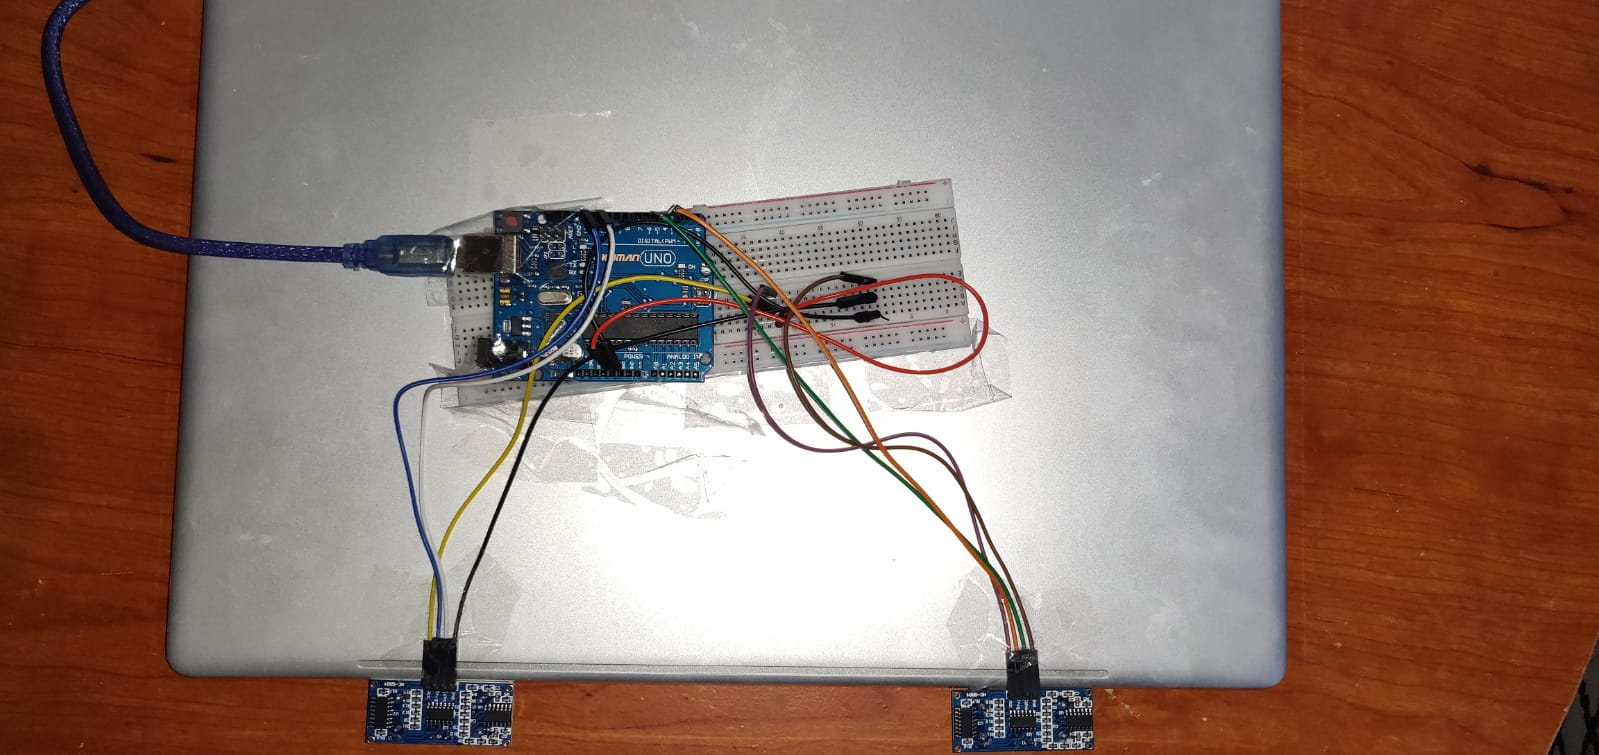
\includegraphics[width=0.5\textwidth]{1.jpeg}
  \caption{The circuit is taped to the back panel of the laptop}
  \label{fig:img1}
\end{figure}

\begin{figure}[h]
\centering
  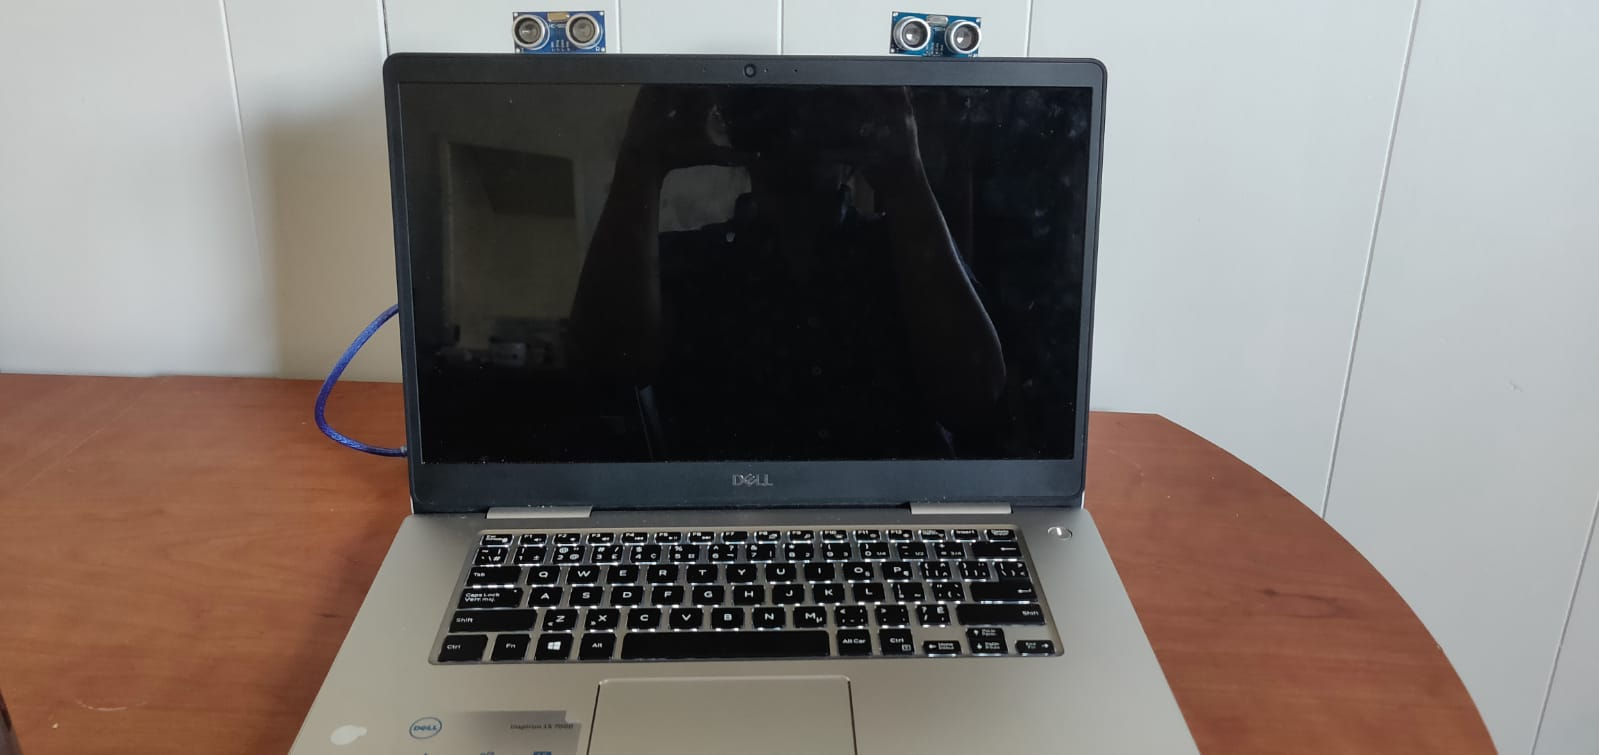
\includegraphics[width=0.5\textwidth]{4.jpeg}
  \caption{The two Ultrasonic sensors to take the input of hand motion}
  \label{fig:img1}
\end{figure}

\begin{figure}[h]
\centering
  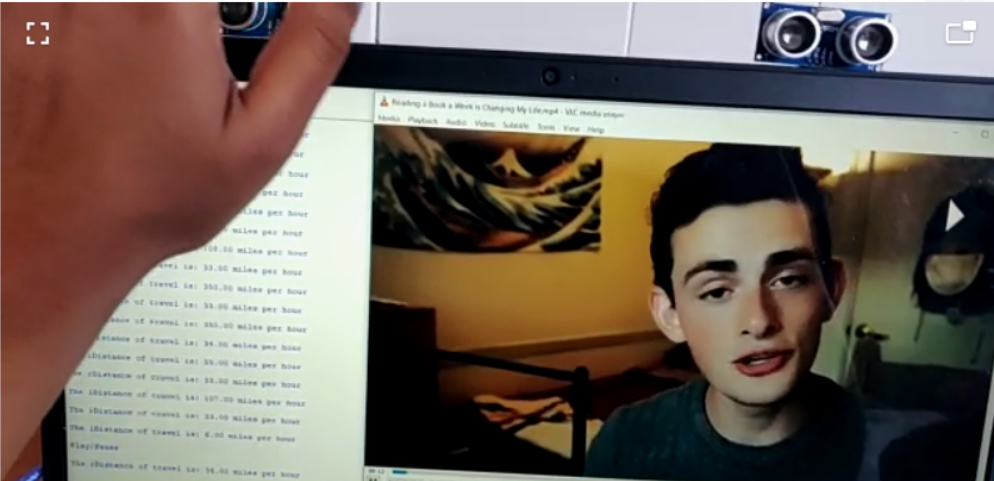
\includegraphics[width=0.5\textwidth]{Play.PNG}
  \caption{Playing the Video}
  \label{fig:img1}
\end{figure}
\begin{figure}[h]
\centering
  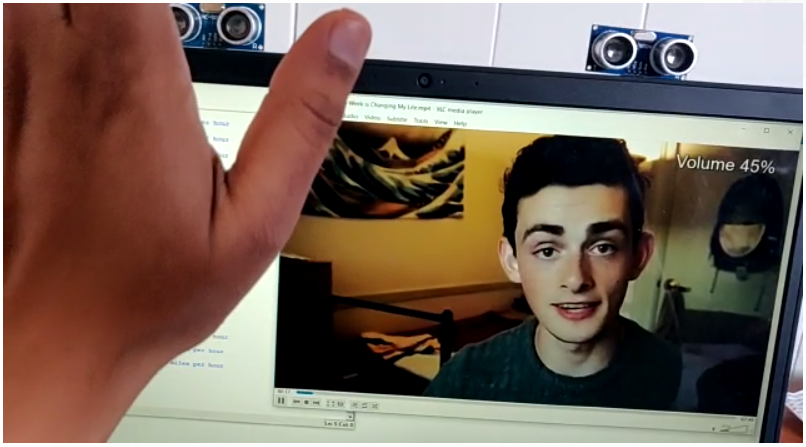
\includegraphics[width=0.5\textwidth]{Decreasevol.PNG}
  \caption{Decreasing the Volume}
  \label{fig:img1}
\end{figure}
\begin{figure}[h]
\centering
  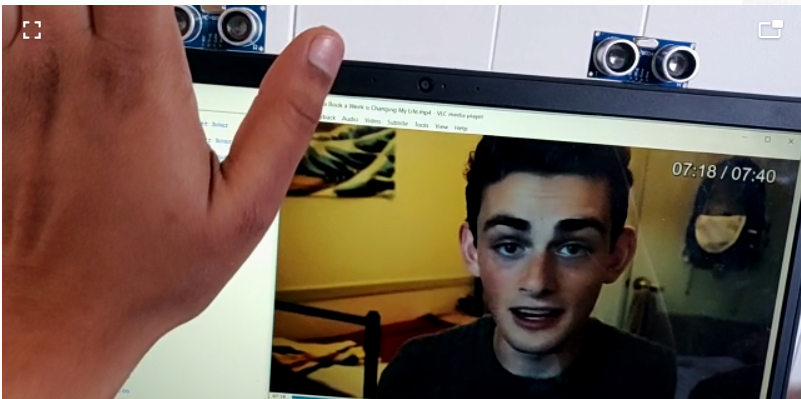
\includegraphics[width=0.5\textwidth]{Forward.PNG}
  \caption{Forwarding the Video}
  \label{fig:img1}
\end{figure}

\newpage
\medskip

\begin{thebibliography}{1}

  \bibitem{notes} Electronics Hub. (2019). Arduino based Hand Gesture Control of Your Computer. [online] Available at: https://www.electronicshub.org/arduino-based-hand-gesture-control-computer/ [Accessed 18 Apr. 2019].

  \bibitem{impj}  Technology, S. and Arduino, A. (2019). Amazing Control Computer Using Hand Motion And Arduino. [online] Hackster.io. Available at: https://www.hackster.io/smart-tech/amazing-control-computer-using-hand-motion-and-arduino-d933f1 [Accessed 18 Apr. 2019].

  \bibitem{norman} Toptechboy.com. (2019). LESSON 17: Measuring the Speed of Sound with Arduino and Ultrasonic Sensor | Technology Tutorials. [online] Available at: http://www.toptechboy.com/arduino/lesson-17-measuring-the-speed-of-sound-with-arduino-and-ultrasonic-sensor/ [Accessed 18 Apr. 2019].

  \bibitem{fo} Create.arduino.cc. (2019). 43 ultrasonic Projects - Arduino Project Hub. [online] Available at: https://create.arduino.cc/projecthub/projects/tags/ultrasonic?page=2 [Accessed 18 Apr. 2019].

  \end{thebibliography}



% that's all folks
\end{document}

